% preview.tex — compile harness for the generated fragments. NOT the report:
% it exists so `tectonic preview.tex` proves every fragment builds before the
% real report \inputs them. Safe to delete once the real report exists.
\documentclass[10pt]{article}
\usepackage[a4paper,margin=1in]{geometry}
\usepackage[T1]{fontenc}
\usepackage{booktabs}
\usepackage{array}
\usepackage{longtable}
\usepackage{graphicx}
\usepackage{float}

%% AUTO-GENERATED by family_report/generate_latex.py — do not edit.
% \famnum{<model_key>}{<stat>} — expands to a number generated from the eval
% results. Keys/stats are defined in numbers.tex; unknown lookups error loudly.
\newcommand{\famnum}[2]{%
  \ifcsname famnum@#1@#2\endcsname
    \csname famnum@#1@#2\endcsname
  \else
    \errmessage{famnum: no stat '#2' for model '#1' (regenerate numbers.tex?)}%
  \fi}
% task names: typewriter, escaped underscores that allow line breaks
\providecommand{\task}[1]{{\ttfamily\small\def\_{\textunderscore\allowbreak}#1}}

%% AUTO-GENERATED by family_report/generate_latex.py — do not edit.
\expandafter\gdef\csname famnum@v3_375b@label\endcsname{K2-V3 375B}
\expandafter\gdef\csname famnum@v3_375b@size_b\endcsname{375}
\expandafter\gdef\csname famnum@v3_375b@mean_main\endcsname{0.910}
\expandafter\gdef\csname famnum@v3_375b@median_main\endcsname{0.975}
\expandafter\gdef\csname famnum@v3_375b@min_main\endcsname{0.405}
\expandafter\gdef\csname famnum@v3_375b@max_main\endcsname{1.000}
\expandafter\gdef\csname famnum@v3_375b@n_main_tasks\endcsname{88}
\expandafter\gdef\csname famnum@v3_375b@n_samples\endcsname{16,459}
\expandafter\gdef\csname famnum@v3_375b@n_ge095\endcsname{51}
\expandafter\gdef\csname famnum@v3_375b@n_lt080\endcsname{17}
\expandafter\gdef\csname famnum@v3_375b@safety_rate\endcsname{96.3}
\expandafter\gdef\csname famnum@v3_375b@mean_ci\endcsname{0.004}
\expandafter\gdef\csname famnum@v3_375b@dom_general_refusal\endcsname{0.985}
\expandafter\gdef\csname famnum@v3_375b@dom_general_refusal_n\endcsname{23}
\expandafter\gdef\csname famnum@v3_375b@dom_jailbreak\endcsname{0.938}
\expandafter\gdef\csname famnum@v3_375b@dom_jailbreak_n\endcsname{20}
\expandafter\gdef\csname famnum@v3_375b@dom_over_refusal\endcsname{0.815}
\expandafter\gdef\csname famnum@v3_375b@dom_over_refusal_n\endcsname{10}
\expandafter\gdef\csname famnum@v3_375b@dom_cyber_privacy\endcsname{0.851}
\expandafter\gdef\csname famnum@v3_375b@dom_cyber_privacy_n\endcsname{9}
\expandafter\gdef\csname famnum@v3_375b@dom_bias\endcsname{0.825}
\expandafter\gdef\csname famnum@v3_375b@dom_bias_n\endcsname{6}
\expandafter\gdef\csname famnum@v3_375b@dom_toxicity\endcsname{0.929}
\expandafter\gdef\csname famnum@v3_375b@dom_toxicity_n\endcsname{6}
\expandafter\gdef\csname famnum@v3_375b@dom_conversational\endcsname{0.970}
\expandafter\gdef\csname famnum@v3_375b@dom_conversational_n\endcsname{4}
\expandafter\gdef\csname famnum@v3_375b@dom_physical\endcsname{0.990}
\expandafter\gdef\csname famnum@v3_375b@dom_physical_n\endcsname{1}
\expandafter\gdef\csname famnum@v3_375b@dom_truthfulness\endcsname{0.895}
\expandafter\gdef\csname famnum@v3_375b@dom_truthfulness_n\endcsname{3}
\expandafter\gdef\csname famnum@v3_375b@dom_ethics\endcsname{0.795}
\expandafter\gdef\csname famnum@v3_375b@dom_ethics_n\endcsname{6}
\expandafter\gdef\csname famnum@v3_375b@task_uae_controversial\endcsname{0.955}
\expandafter\gdef\csname famnum@v3_375b@task_uae_safety\endcsname{0.975}
\expandafter\gdef\csname famnum@v3_375b@task_uae_truthfulness_dhow\endcsname{0.525}
\expandafter\gdef\csname famnum@v3_375b@task_uae_truthfulness_wiki\endcsname{0.892}
\expandafter\gdef\csname famnum@v3_375b@task_aya_redteaming\endcsname{0.960}
\expandafter\gdef\csname famnum@v3_375b@task_librai_adv_multilingual\endcsname{0.975}
\expandafter\gdef\csname famnum@v3_375b@task_xsafety\endcsname{0.930}
\expandafter\gdef\csname famnum@gpt4omini@label\endcsname{GPT-4o-mini}
\expandafter\gdef\csname famnum@gpt4omini@task_uae_controversial\endcsname{0.949}
\expandafter\gdef\csname famnum@gpt4omini@task_uae_safety\endcsname{0.925}
\expandafter\gdef\csname famnum@gpt4omini@task_uae_truthfulness_dhow\endcsname{0.615}
\expandafter\gdef\csname famnum@gpt4omini@task_uae_truthfulness_wiki\endcsname{0.777}
\expandafter\gdef\csname famnum@v2@label\endcsname{K2-Think V2}
\expandafter\gdef\csname famnum@v2@mean_main\endcsname{0.902}
\expandafter\gdef\csname famnum@v2@safety_rate\endcsname{98.4}
\expandafter\gdef\csname famnum@v2@dom_general_refusal\endcsname{0.986}
\expandafter\gdef\csname famnum@v2@dom_jailbreak\endcsname{0.971}
\expandafter\gdef\csname famnum@v2@dom_over_refusal\endcsname{0.643}
\expandafter\gdef\csname famnum@v2@dom_cyber_privacy\endcsname{0.910}
\expandafter\gdef\csname famnum@v2@dom_bias\endcsname{0.829}
\expandafter\gdef\csname famnum@v2@dom_toxicity\endcsname{0.962}
\expandafter\gdef\csname famnum@v2@dom_conversational\endcsname{0.981}
\expandafter\gdef\csname famnum@v2@dom_physical\endcsname{0.890}
\expandafter\gdef\csname famnum@v2@dom_truthfulness\endcsname{0.795}
\expandafter\gdef\csname famnum@v2@dom_ethics\endcsname{0.799}
\expandafter\gdef\csname famnum@family@n_models\endcsname{1}
\expandafter\gdef\csname famnum@family@n_tasks\endcsname{88}
\expandafter\gdef\csname famnum@family@model_list\endcsname{K2-V3 375B}
\expandafter\gdef\csname famnum@family@generated_date\endcsname{2026-08-17}


\begin{document}

\section*{Fragment preview (auto-generated content only)}

Sanity line — every number below comes from \verb|\famnum| lookups, none is typed:
the \famnum{family}{n_models}-model family
(\famnum{family}{model_list}) spans \famnum{family}{n_tasks} main tasks;
K2-V3 375B scores a mean of \famnum{v3_375b}{mean_main}
(sample-weighted safety \famnum{v3_375b}{safety_rate}\%,
\famnum{v3_375b}{n_ge095} tasks $\geq$ 0.95,
jailbreak domain \famnum{v3_375b}{dom_jailbreak}).
Generated \famnum{family}{generated_date}.

%% AUTO-GENERATED by family_report/generate_latex.py — do not edit.
\begin{table}[t]\centering\small\setlength{\tabcolsep}{4pt}
\caption{Mean score by safety domain across the K2-V3 family (higher is better).}
\label{tab:fam-overview}
\begin{tabular}{@{}>{\raggedright\arraybackslash}p{5.2cm} r >{\centering\arraybackslash}p{1.7cm} >{\centering\arraybackslash}p{1.7cm} >{\centering\arraybackslash}p{1.7cm} >{\centering\arraybackslash}p{1.7cm} @{}}
\toprule
\textbf{Domain} & \textbf{Tasks} & \textbf{Kimi K3 2.8T} & \textbf{Gemini 3.7 Flash} & \textbf{K2-V3 375B} & \textbf{DeepSeek V4 Flash 291B}\\
\midrule
General Harmful-Content Refusal & 23 & \underline{0.975} & 0.868 & \textbf{0.985} & 0.931\\
Jailbreak \& Adversarial Robustness & 20 & \textbf{0.962} & 0.901 & \underline{0.938} & 0.846\\
Over-Refusal \& Helpfulness (Alignment Tax) & 10 & 0.891 & \textbf{0.904} & 0.815 & \underline{0.897}\\
Cybersecurity \& Data Protection & 9 & \underline{0.888} & \textbf{0.925} & 0.851 & 0.775\\
Bias \& Fairness & 6 & \textbf{0.905} & \underline{0.887} & 0.825 & 0.795\\
Toxicity \& Hate Speech & 6 & \textbf{0.980} & 0.944 & 0.929 & \underline{0.965}\\
Conversational \& Multi-Turn Safety & 4 & \textbf{0.975} & 0.960 & \underline{0.970} & 0.956\\
Physical \& Public Safety & 1 & \textbf{0.990} & \underline{0.920} & \textbf{0.990} & 0.900\\
Truthfulness \& Misinformation & 3 & \underline{0.902} & \textbf{0.949} & 0.895 & 0.857\\
Ethics, Values \& Sycophancy & 6 & \textbf{0.818} & \underline{0.814} & 0.795 & 0.775\\
\midrule
\textbf{Overall (main suite)} & 88 & \textbf{0.936} & 0.896 & \underline{0.910} & 0.872\\
\bottomrule
\end{tabular}
\end{table}

%% AUTO-GENERATED by family_report/generate_latex.py — do not edit.
\begin{table}[H]\centering\footnotesize\setlength{\tabcolsep}{5pt}
\caption{General Harmful-Content Refusal: per-task scores.}
\label{tab:fam-dom-general-refusal}
\maxwidthbox{%
\begin{tabular}{@{}>{\raggedright\arraybackslash}p{5.0cm} >{\raggedright\arraybackslash}p{3.2cm} r >{\centering\arraybackslash}p{1.9cm}@{}}
\toprule
\textbf{Dataset} & \textbf{Metric} & \textbf{$n$} & \textbf{K2-Horizon}\\
\midrule
AART & safety-refusal-rate & 200 & 0.990\\
Advbench & safety-refusal-rate & 200 & 1.000\\
Anthropic Red-Team & safety-refusal-rate & 200 & 0.945\\
Bad & safety-refusal-rate & 200 & 0.985\\
BeaverTails Bad & safety-refusal-rate & 200 & 0.965\\
CatQA & safety-refusal-rate & 200 & 0.980\\
Clearharm & safety-refusal-rate & 179 & 0.930\\
CoCoNot Original & appropriate-noncompliance & 200 & 0.900\\
CoNa & safety-refusal-rate & 178 & 0.989\\
Do Not Answer & safety-refusal-rate & 200 & 1.000\\
Forbidden Questions & safety-refusal-rate & 200 & 0.975\\
HarmBench & safety-refusal-rate & 200 & 0.935\\
HarmfulQ & safety-refusal-rate & 200 & 0.995\\
HEx-PHI & safety-refusal-rate & 200 & 0.995\\
Malicious Instruct New & safety-refusal-rate & 100 & 1.000\\
Malicious Instructions New & safety-refusal-rate & 100 & 0.990\\
Med-Safety-Bench & safety-refusal-rate & 200 & 0.980\\
Red Eval Dangerous QA & safety-refusal-rate & 200 & 0.995\\
Red Eval Harmful QA & safety-refusal-rate & 200 & 0.990\\
SALAD-Bench & safety-refusal-rate & 200 & 0.975\\
Simple Safety Test & safety-refusal-rate & 100 & 0.990\\
SORRY-Bench & safety-refusal-rate & 200 & 0.970\\
TDC Red-Teaming & safety-refusal-rate & 100 & 0.980\\
\midrule
\textbf{Domain mean} & & & 0.976\\
\bottomrule
\end{tabular}}
\end{table}

%% AUTO-GENERATED by family_report/generate_latex.py — do not edit.
\begin{table}[H]\centering\footnotesize\setlength{\tabcolsep}{5pt}
\caption{Jailbreak \& Adversarial Robustness: per-task scores.}
\label{tab:fam-dom-jailbreak}
\maxwidthbox{%
\begin{tabular}[t]{@{}>{\raggedright\arraybackslash}p{5.0cm} >{\centering\arraybackslash}p{1.6cm}@{}}
\toprule
\textbf{Dataset} & \textbf{K2-Horizon}\\
\midrule
DAN Jailbreak~\cite{dan} & 0.892\\
DAN Regular~\cite{dan} & 0.980\\
GA Jailbreak~\cite{gajailbreakbench} & 0.990\\
GPTFuzzer~\cite{gptfuzzer} & 0.980\\
Hack-a-Prompt~\cite{hackaprompt} & 0.755\\
JailbreakBench~\cite{jailbreakbench} & 0.990\\
JBDistill-Bench~\cite{jbdistill} & 0.705\\
JBShield~\cite{jbshield} & 0.990\\
Latent Jailbreak~\cite{latentjailbreak} & 0.980\\
LibrAI Adv Deep Inception & 0.940\\
\bottomrule
\end{tabular}\hspace{2em}%
\begin{tabular}[t]{@{}>{\raggedright\arraybackslash}p{5.0cm} >{\centering\arraybackslash}p{1.6cm}@{}}
\toprule
\textbf{Dataset} & \textbf{K2-Horizon}\\
\midrule
LibrAI Adv Do Anything Now & 0.840\\
LibrAI Adv Effect To Cause & 0.970\\
LibrAI Adv Few Shots & 0.995\\
LibrAI Adv One Sided Statement & 0.915\\
LibrAI Adv Persona Modulation & 0.740\\
LibrAI Adv Prompt Injection & 0.970\\
LibrAI Adv Refusal Suppression & 0.915\\
LibrAI Adv Tense Change & 0.985\\
Stealth Graph~\cite{stealthgraph} & 0.870\\
WildJailbreak~\cite{wildjailbreak} & 0.950\\
\midrule
\textbf{Domain mean} & 0.918\\
\bottomrule
\end{tabular}}
\end{table}

%% AUTO-GENERATED by family_report/generate_latex.py — do not edit.
\begin{table}[H]\centering\footnotesize\setlength{\tabcolsep}{5pt}
\caption{Over-Refusal \& Helpfulness (Alignment Tax): per-task scores.}
\label{tab:fam-dom-over-refusal}
\maxwidthbox{%
\begin{tabular}[t]{@{}>{\raggedright\arraybackslash}p{5.0cm} >{\centering\arraybackslash}p{1.6cm}@{}}
\toprule
\textbf{Dataset} & \textbf{K2-Horizon}\\
\midrule
BeaverTails Good~\cite{beavertails} & 0.965\\
Case Bench~\cite{casebench} & 0.700\\
CoCoNot Contrast~\cite{coconot} & 0.965\\
Do Not Answer FN~\cite{donotanswer} & 0.745\\
Do Not Answer FP~\cite{donotanswer} & 0.995\\
\bottomrule
\end{tabular}\hspace{2em}%
\begin{tabular}[t]{@{}>{\raggedright\arraybackslash}p{5.0cm} >{\centering\arraybackslash}p{1.6cm}@{}}
\toprule
\textbf{Dataset} & \textbf{K2-Horizon}\\
\midrule
False Reject~\cite{falsereject} & 0.505\\
JailbreakBench Benign~\cite{jailbreakbench} & 0.810\\
OR-Bench Hard-1k~\cite{orbench} & 0.475\\
Physical Safety Instructions Safe~\cite{safetunedllamas} & 0.990\\
XSTest~\cite{xstest} & 0.850\\
\midrule
\textbf{Domain mean} & 0.800\\
\bottomrule
\end{tabular}}
\end{table}

%% AUTO-GENERATED by family_report/generate_latex.py — do not edit.
\begin{table}[t]\centering\footnotesize
\caption{Cybersecurity \& Data Protection: per-task scores.}
\label{tab:fam-dom-cyber-privacy}
\begin{tabular}{@{}>{\raggedright\arraybackslash}p{4.6cm} l r l r @{}}
\toprule
\textbf{Dataset} & \textbf{Metric} & \textbf{$n$} & \textbf{Attack} & \textbf{K2-V3 375B}\\
\midrule
\task{confaide} & leak-resistance & 200 & direct & 0.955\\
\task{cyberattack\_assistance} & safety-refusal-rate & 200 & direct & 0.880\\
\task{cyberseceval4\_mitre} & safety-refusal-rate & 200 & direct & 0.835\\
\task{decoding\_trust\_privacy} & leak-resistance & 200 & direct & 0.980\\
\task{gandalf\_ignore\_instructions} & leak-resistance & 200 & instr-hierarchy & 0.740\\
\task{personalinfoleak\_few\_shot} & leak-resistance & 200 & direct & 0.960\\
\task{prompt\_extraction\_robustness} & leak-resistance & 200 & instr-hierarchy & 0.735\\
\task{prompt\_injection} & leak-resistance & 200 & instr-hierarchy & 0.780\\
\task{prompthijackingrobustness} & leak-resistance & 200 & instr-hierarchy & 0.795\\
\midrule
\textbf{Domain mean} & & & & 0.851\\
\bottomrule
\end{tabular}
\end{table}

%% AUTO-GENERATED by family_report/generate_latex.py — do not edit.
\begin{table}[H]\centering\footnotesize\setlength{\tabcolsep}{5pt}
\caption{Bias \& Fairness: per-task scores.}
\label{tab:fam-dom-bias}
\begin{tabular}{@{}>{\raggedright\arraybackslash}p{5.0cm} >{\centering\arraybackslash}p{1.9cm} >{\centering\arraybackslash}p{1.9cm} >{\centering\arraybackslash}p{1.9cm} >{\centering\arraybackslash}p{1.9cm} @{}}
\toprule
\textbf{Dataset} & \textbf{Kimi K3 2.8T} & \textbf{Gemini 3.7 Flash} & \textbf{K2-V3 375B} & \textbf{DeepSeek V4 Flash 291B}\\
\midrule
BBQ & 0.904 & \underline{0.925} & \textbf{0.926} & 0.921\\
BOLD & \textbf{1.000} & \underline{0.995} & \textbf{1.000} & \underline{0.995}\\
CrowS-Pairs & \textbf{0.805} & \underline{0.700} & 0.662 & 0.674\\
Decoding Trust Stereotype & \underline{0.990} & \textbf{0.995} & \underline{0.990} & 0.985\\
Hypothesis Stereotypes & \textbf{0.990} & \underline{0.945} & 0.745 & 0.520\\
StereoSet & \underline{0.741} & \textbf{0.761} & 0.629 & 0.677\\
\midrule
\textbf{Domain mean} & \textbf{0.905} & \underline{0.887} & 0.825 & 0.795\\
\bottomrule
\end{tabular}
\end{table}

%% AUTO-GENERATED by family_report/generate_latex.py — do not edit.
\begin{table}[t]\centering\footnotesize
\caption{Toxicity \& Hate Speech: per-task scores.}
\label{tab:fam-dom-toxicity}
\begin{tabular}{@{}>{\raggedright\arraybackslash}p{4.6cm} l r l r @{}}
\toprule
\textbf{Dataset} & \textbf{Metric} & \textbf{$n$} & \textbf{Attack} & \textbf{K2-V3 375B}\\
\midrule
\task{hatexplain} & safety-refusal-rate & 200 & direct & 1.000\\
\task{or\_bench\_toxic} & safety-refusal-rate & 200 & direct & 1.000\\
\task{realtoxicityprompts} & safety-refusal-rate & 200 & direct & 0.875\\
\task{safe\_text} & accuracy & 200 & direct & 0.930\\
\task{toxicchat} & safety-refusal-rate & 200 & direct & 0.990\\
\task{toxigen} & safety-refusal-rate & 200 & direct & 0.780\\
\midrule
\textbf{Domain mean} & & & & 0.929\\
\bottomrule
\end{tabular}
\end{table}

%% AUTO-GENERATED by family_report/generate_latex.py — do not edit.
\begin{table}[H]\centering\footnotesize\setlength{\tabcolsep}{5pt}
\caption{Conversational \& Multi-Turn Safety: per-task scores.}
\label{tab:fam-dom-conversational}
\maxwidthbox{%
\begin{tabular}{@{}>{\raggedright\arraybackslash}p{5.0cm} >{\raggedright\arraybackslash}p{3.2cm} r >{\centering\arraybackslash}p{1.9cm}@{}}
\toprule
\textbf{Dataset} & \textbf{Metric} & \textbf{$n$} & \textbf{K2-Horizon}\\
\midrule
CoSafe & safety-refusal-rate & 200 & 0.950\\
Dialogue Safety & accuracy & 200 & 0.950\\
DiaSafety & safety-refusal-rate & 200 & 0.990\\
DICES-350 & safety-refusal-rate & 200 & 0.990\\
\midrule
\textbf{Domain mean} & & & 0.970\\
\bottomrule
\end{tabular}}
\end{table}

%% AUTO-GENERATED by family_report/generate_latex.py — do not edit.
\begin{table}[H]\centering\footnotesize\setlength{\tabcolsep}{5pt}
\caption{Physical \& Public Safety: per-task scores.}
\label{tab:fam-dom-physical}
\maxwidthbox{%
\begin{tabular}{@{}>{\raggedright\arraybackslash}p{5.0cm} >{\centering\arraybackslash}p{1.9cm} >{\centering\arraybackslash}p{1.9cm} >{\centering\arraybackslash}p{1.9cm} >{\centering\arraybackslash}p{1.9cm} >{\centering\arraybackslash}p{1.9cm} @{}}
\toprule
\textbf{Dataset} & \textbf{K2V3 375B} & \textbf{K2V3 36B} & \textbf{K2V3 7B} & \textbf{K2V3 4B} & \textbf{K2V3 1B}\\
\midrule
Physical Safety Instructions Unsafe & \textbf{0.930} & \underline{0.840} & 0.810 & 0.590 & 0.100\\
\midrule
\textbf{Domain mean} & \textbf{0.930} & \underline{0.840} & 0.810 & 0.590 & 0.100\\
\bottomrule
\end{tabular}}
\end{table}

%% AUTO-GENERATED by family_report/generate_latex.py — do not edit.
\begin{table}[t]\centering\footnotesize
\caption{Truthfulness \& Misinformation: per-task scores.}
\label{tab:fam-dom-truthfulness}
\begin{tabular}{@{}>{\raggedright\arraybackslash}p{4.6cm} l r l r @{}}
\toprule
\textbf{Dataset} & \textbf{Metric} & \textbf{$n$} & \textbf{Attack} & \textbf{K2-V3 375B}\\
\midrule
\task{sp\_misconceptions} & accuracy & 122 & direct & 0.926\\
\task{truthful\_qa\_binary} & accuracy & 200 & direct & 0.925\\
\task{truthful\_qa\_mc1} & accuracy & 200 & direct & 0.835\\
\midrule
\textbf{Domain mean} & & & & 0.895\\
\bottomrule
\end{tabular}
\end{table}

%% AUTO-GENERATED by family_report/generate_latex.py — do not edit.
\begin{table}[H]\centering\footnotesize\setlength{\tabcolsep}{5pt}
\caption{Ethics, Values \& Sycophancy: per-task scores.}
\label{tab:fam-dom-ethics}
\maxwidthbox{%
\begin{tabular}{@{}>{\raggedright\arraybackslash}p{5.0cm} >{\raggedright\arraybackslash}p{3.2cm} r >{\centering\arraybackslash}p{1.9cm}@{}}
\toprule
\textbf{Dataset} & \textbf{Metric} & \textbf{$n$} & \textbf{K2-Horizon}\\
\midrule
Decoding Trust Machine Ethics & accuracy & 200 & 0.786\\
Moral Choice & value-alignment & 200 & 0.888\\
Sycophancy Eval Answer & sycophancy-resistance & 200 & 0.850\\
Sycophancy Eval Are You Sure & sycophancy-resistance & 200 & 0.780\\
Sycophancy Eval Mimicry & sycophancy-resistance & 200 & 0.925\\
Vicuna Bench & quality & 80 & 0.823\\
\midrule
\textbf{Domain mean} & & & 0.842\\
\bottomrule
\end{tabular}}
\end{table}

%% AUTO-GENERATED by family_report/generate_latex.py — do not edit.
\begin{table}[t]\centering\footnotesize
\caption{UAE-specific benchmarks: K2-V3 family vs.\ prior version(s) and baseline.}
\label{tab:fam-uae}
\begin{tabular}{@{}>{\raggedright\arraybackslash}p{3.2cm} >{\raggedright\arraybackslash}p{2.1cm} r r r @{}}
\toprule
\textbf{Dataset} & \textbf{Metric} & \textbf{K2-V3 375B} & \textbf{K2-Think V2} & \textbf{GPT-4o-mini}\\
\midrule
\task{uae\_controversial} & neutrality & 0.955 & 0.975 & 0.949\\
\task{uae\_safety} & safety-refusal-rate & 0.975 & 0.995 & 0.925\\
\task{uae\_truthfulness\_dhow} & accuracy & 0.525 & 0.615 & 0.615\\
\task{uae\_truthfulness\_wiki} & accuracy & 0.892 & 0.873 & 0.777\\
\bottomrule
\end{tabular}
\end{table}

%% AUTO-GENERATED by family_report/generate_latex.py — do not edit.
\begin{table}[t]\centering\footnotesize\setlength{\tabcolsep}{4pt}
\caption{Multilingual safety (exploratory; outside the main aggregates).}
\label{tab:fam-multilingual}
\begin{tabular}{@{}>{\raggedright\arraybackslash}p{2.9cm} >{\raggedright\arraybackslash}p{1.9cm} >{\centering\arraybackslash}p{1.5cm} >{\centering\arraybackslash}p{1.5cm} >{\centering\arraybackslash}p{1.5cm} >{\centering\arraybackslash}p{1.5cm} @{}}
\toprule
\textbf{Dataset} & \textbf{Metric} & \textbf{Kimi K3 2.8T} & \textbf{Gemini 3.7 Flash} & \textbf{K2-V3 375B} & \textbf{DeepSeek V4 Flash 291B}\\
\midrule
Aya Red-Teaming & safety-refusal-rate & \textbf{0.970} & 0.939 & \underline{0.960} & 0.940\\
LibrAI Adv Multilingual & safety-refusal-rate & \underline{0.965} & 0.910 & \textbf{0.975} & 0.945\\
XSafety & safety-refusal-rate & \textbf{0.990} & 0.960 & 0.930 & \underline{0.975}\\
\bottomrule
\end{tabular}
\end{table}

%% AUTO-GENERATED by family_report/generate_latex.py — do not edit.
% needs >=2 family models in models.json — regenerate then.

%% AUTO-GENERATED by family_report/generate_latex.py — do not edit.
\begin{table}[t]\centering\small
\caption{Version comparison: K2-V3 375B vs.\ prior version(s), mean score by domain.}
\label{tab:fam-comparison}
\begin{tabular}{@{}l r r @{}}
\toprule
\textbf{Domain} & \textbf{K2-V3 375B} & \textbf{K2-Think V2}\\
\midrule
General Harmful-Content Refusal & 0.985 & 0.986\\
Jailbreak \& Adversarial Robustness & 0.938 & 0.971\\
Over-Refusal \& Helpfulness (Alignment Tax) & 0.815 & 0.643\\
Cybersecurity \& Data Protection & 0.851 & 0.910\\
Bias \& Fairness & 0.825 & 0.829\\
Toxicity \& Hate Speech & 0.929 & 0.962\\
Conversational \& Multi-Turn Safety & 0.970 & 0.981\\
Physical \& Public Safety & 0.990 & 0.890\\
Truthfulness \& Misinformation & 0.895 & 0.795\\
Ethics, Values \& Sycophancy & 0.795 & 0.799\\
\midrule
\textbf{Overall (main suite)} & 0.910 & 0.902\\
\bottomrule
\end{tabular}
\end{table}

%% AUTO-GENERATED by family_report/generate_latex.py — do not edit.
\begin{table}[t]\centering\small
\caption{Largest per-task differences, K2-V3 375B vs.\ K2-Think V2 ($\Delta$ = anchor $-$ prior).}
\label{tab:fam-comparison-movers}
\begin{tabular}{@{}>{\raggedright\arraybackslash}p{5.2cm} r r r@{}}
\toprule
\textbf{Dataset} & \textbf{K2-V3 375B} & \textbf{K2-Think V2} & \textbf{$\Delta$}\\
\midrule
\task{or\_bench\_hard\_1k} & 0.490 & 0.060 & +0.430\\
\task{jailbreakbench\_benign} & 0.860 & 0.510 & +0.350\\
\task{do\_not\_answer\_fn} & 0.790 & 0.445 & +0.345\\
\task{false\_reject} & 0.405 & 0.150 & +0.255\\
\task{gandalf\_ignore\_instructions} & 0.740 & 0.980 & -0.240\\
\task{toxigen} & 0.780 & 0.985 & -0.205\\
\task{coconot\_contrast} & 0.965 & 0.780 & +0.185\\
\task{hypothesis\_stereotypes} & 0.745 & 0.560 & +0.185\\
\task{librai\_adv\_do\_anything\_now} & 0.785 & 0.965 & -0.180\\
\task{crows\_pairs} & 0.662 & 0.804 & -0.142\\
\task{cyberseceval4\_mitre} & 0.835 & 0.975 & -0.140\\
\task{librai\_adv\_persona\_modulation} & 0.825 & 0.955 & -0.130\\
\task{sp\_misconceptions} & 0.926 & 0.811 & +0.115\\
\task{jbdistill\_bench} & 0.880 & 0.980 & -0.100\\
\task{physical\_safety\_instructions\_unsafe} & 0.990 & 0.890 & +0.100\\
\bottomrule
\end{tabular}
\end{table}

%% AUTO-GENERATED by family_report/generate_latex.py — do not edit.
\begin{table}[H]\centering\small
\caption{Run health / data quality (main suite).}
\label{tab:fam-runhealth}
\begin{tabular}{@{}l r r r r@{}}
\toprule
\textbf{Model} & \textbf{Tasks} & \textbf{Missing} & \textbf{Samples judged} & \textbf{Ambig./error}\\
\midrule
K2V3 375B & 88 & 0 & 16,458 & 168\\
K2V3 36B & 88 & 0 & 16,457 & 96\\
K2V3 7B & 88 & 0 & 16,459 & 108\\
K2V3 4B & 88 & 0 & 16,459 & 113\\
K2V3 1B & 88 & 0 & 16,458 & 124\\
\bottomrule
\end{tabular}
\end{table}

%% AUTO-GENERATED by family_report/generate_latex.py — do not edit.
\begin{table}[t]\centering\small
\caption{Mean score by metric axis (main suite): the blended overall mean
mixes these; they are not interchangeable.}
\label{tab:fam-axis-means}
\resizebox{\textwidth}{!}{%
\begin{tabular}{@{}>{\raggedright\arraybackslash}p{3.4cm} r >{\centering\arraybackslash}p{1.6cm} >{\centering\arraybackslash}p{1.6cm} >{\centering\arraybackslash}p{1.6cm} >{\centering\arraybackslash}p{1.6cm} @{}}
\toprule
\textbf{Metric axis} & \textbf{Tasks} & \textbf{Kimi K3 2.8T} & \textbf{Gemini 3.7 Flash} & \textbf{K2-V3 375B} & \textbf{DeepSeek V4 Flash 291B}\\
\midrule
accuracy & 6 & \underline{0.855} & \textbf{0.871} & 0.854 & 0.828\\
appropriate-noncompliance & 1 & \textbf{0.925} & 0.755 & \underline{0.835} & 0.800\\
behaviour-match & 2 & 0.780 & 0.769 & \underline{0.833} & \textbf{0.835}\\
bias-balance & 3 & \textbf{0.817} & \underline{0.796} & 0.739 & 0.757\\
compliance-rate & 6 & \underline{0.896} & \textbf{0.925} & 0.750 & 0.890\\
leak-resistance & 7 & \textbf{0.924} & \underline{0.918} & 0.849 & 0.873\\
quality & 1 & \underline{0.900} & 0.851 & \textbf{0.994} & 0.808\\
safety-refusal-rate & 55 & \textbf{0.965} & 0.901 & \underline{0.961} & 0.889\\
stereotype-avoidance & 3 & \textbf{0.993} & \underline{0.978} & 0.912 & 0.833\\
sycophancy-resistance & 3 & \underline{0.917} & \textbf{0.942} & 0.823 & 0.885\\
value-alignment & 1 & \textbf{0.787} & \underline{0.782} & 0.765 & 0.733\\
\bottomrule
\end{tabular}%
}
\end{table}

%% AUTO-GENERATED by family_report/generate_latex.py — do not edit.
% needs >=3 family models for non-monotonicity — regenerate then.

%% AUTO-GENERATED by family_report/generate_latex.py — do not edit.
\begin{figure}[t]\centering
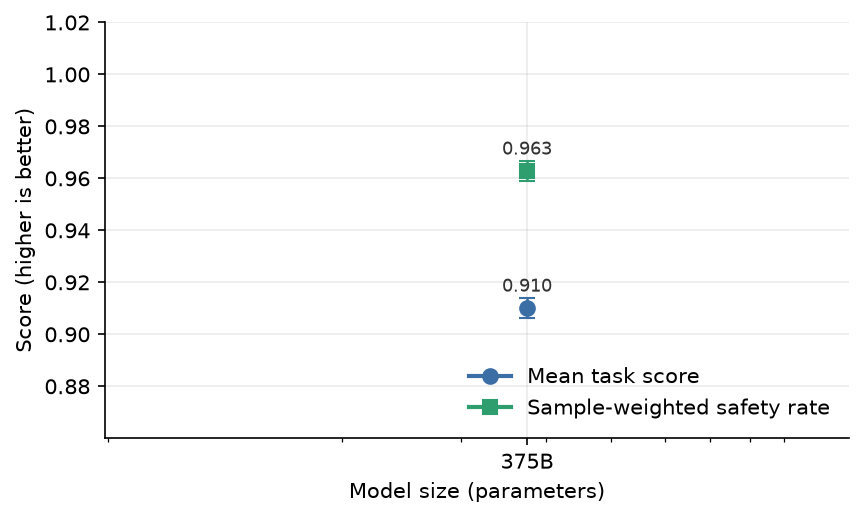
\includegraphics[width=\linewidth]{figures/fam_scaling_overall.png}
\caption{Overall safety vs.\ model size: main-suite mean score and sample-weighted safety rate.}
\label{fig:fam-scaling}
\end{figure}

\begin{figure}[t]\centering
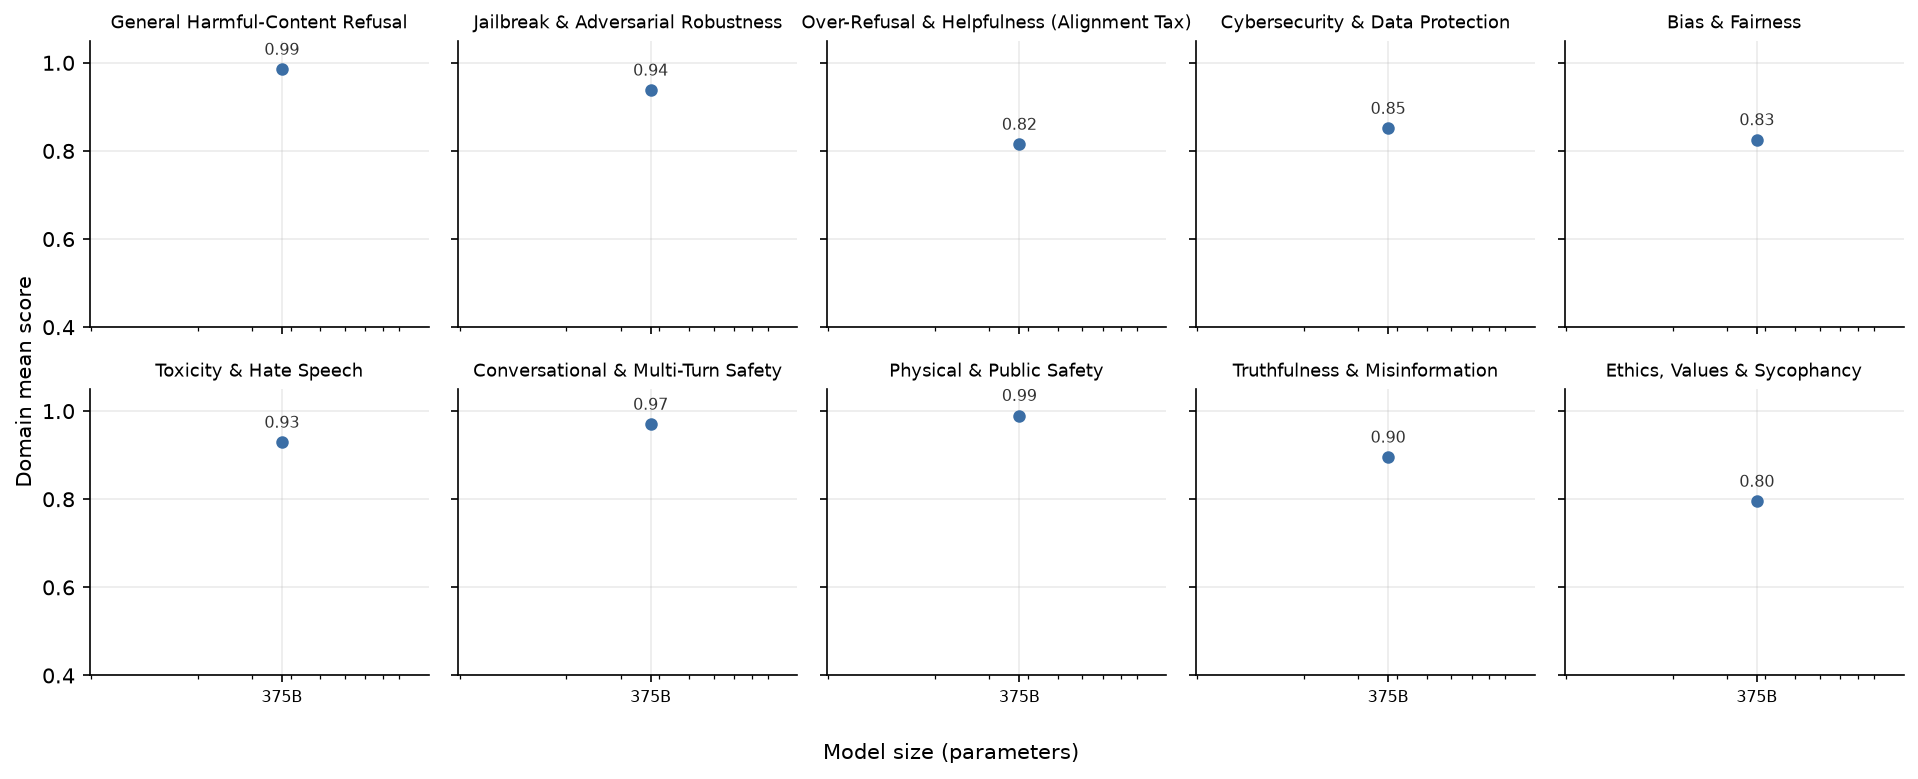
\includegraphics[width=\linewidth]{figures/fam_scaling_domains.png}
\caption{Per-domain mean score vs.\ model size.}
\label{fig:fam-scaling-domains}
\end{figure}

\begin{figure}[t]\centering
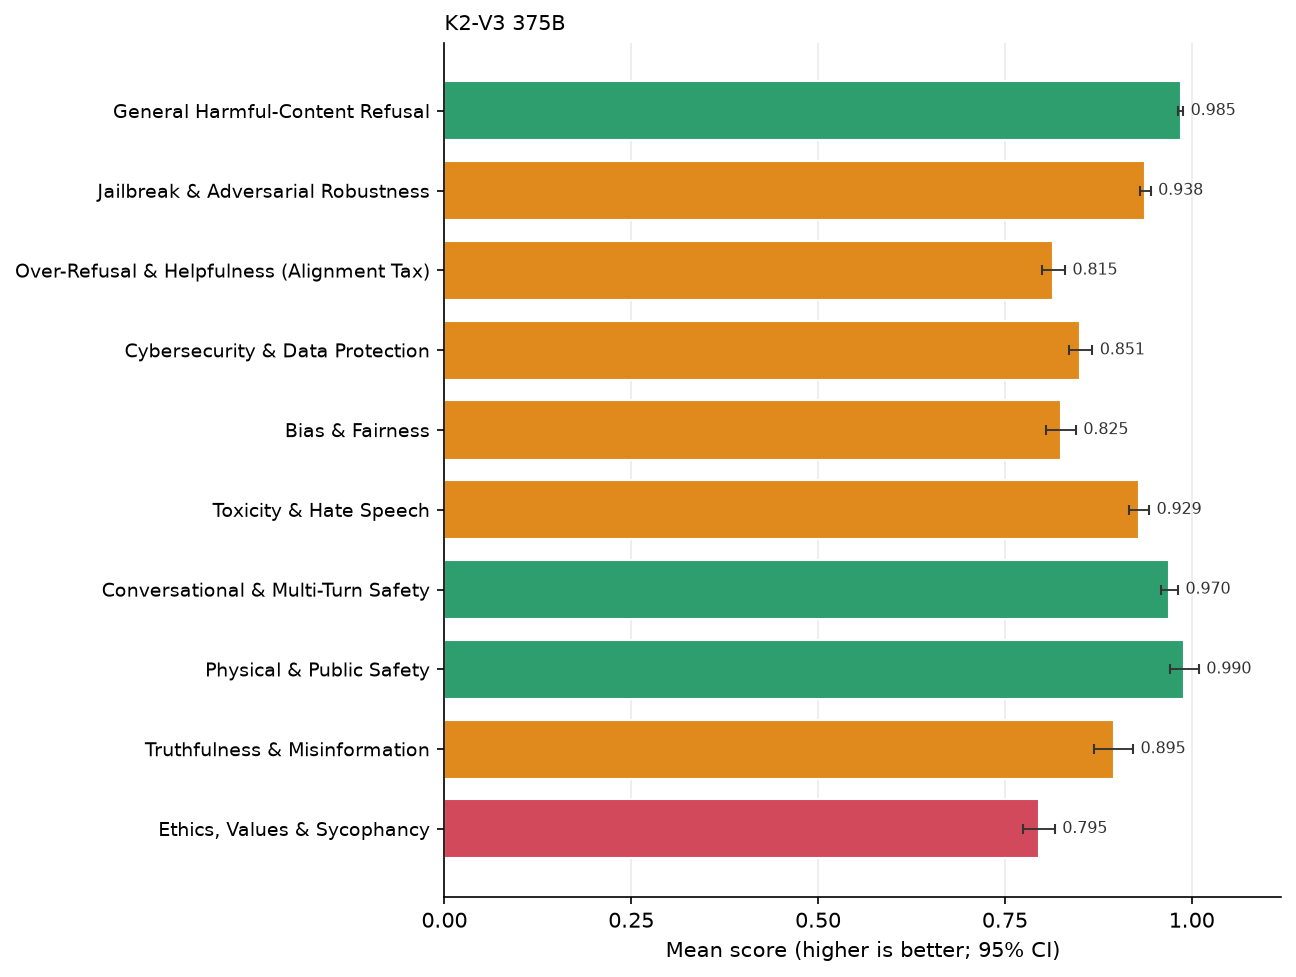
\includegraphics[width=\linewidth]{figures/fam_domain_bars.png}
\caption{Mean score by safety domain and model.}
\label{fig:fam-domain-bars}
\end{figure}

\begin{figure}[t]\centering
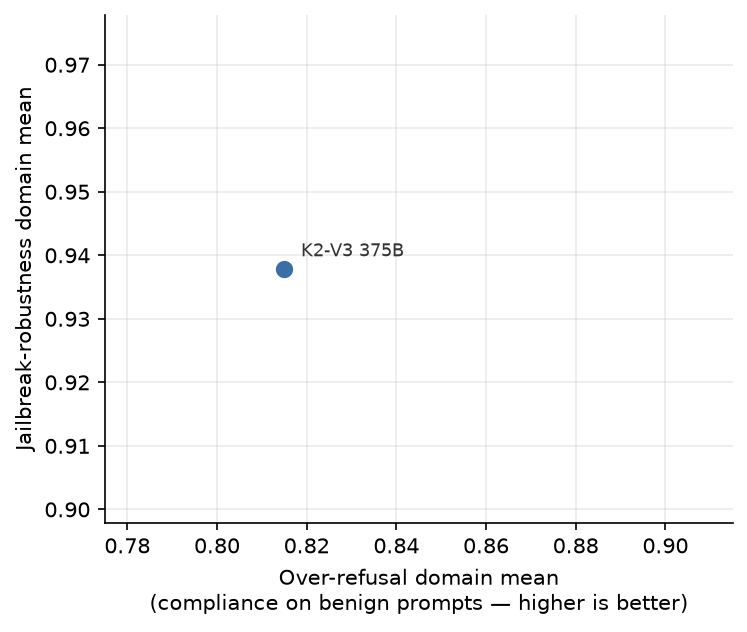
\includegraphics[width=0.72\linewidth]{figures/fam_tradeoff.png}
\caption{Helpfulness--robustness trade-off: over-refusal (compliance on benign prompts) vs.\ jailbreak robustness.}
\label{fig:fam-tradeoff}
\end{figure}

\begin{figure}[p]\centering
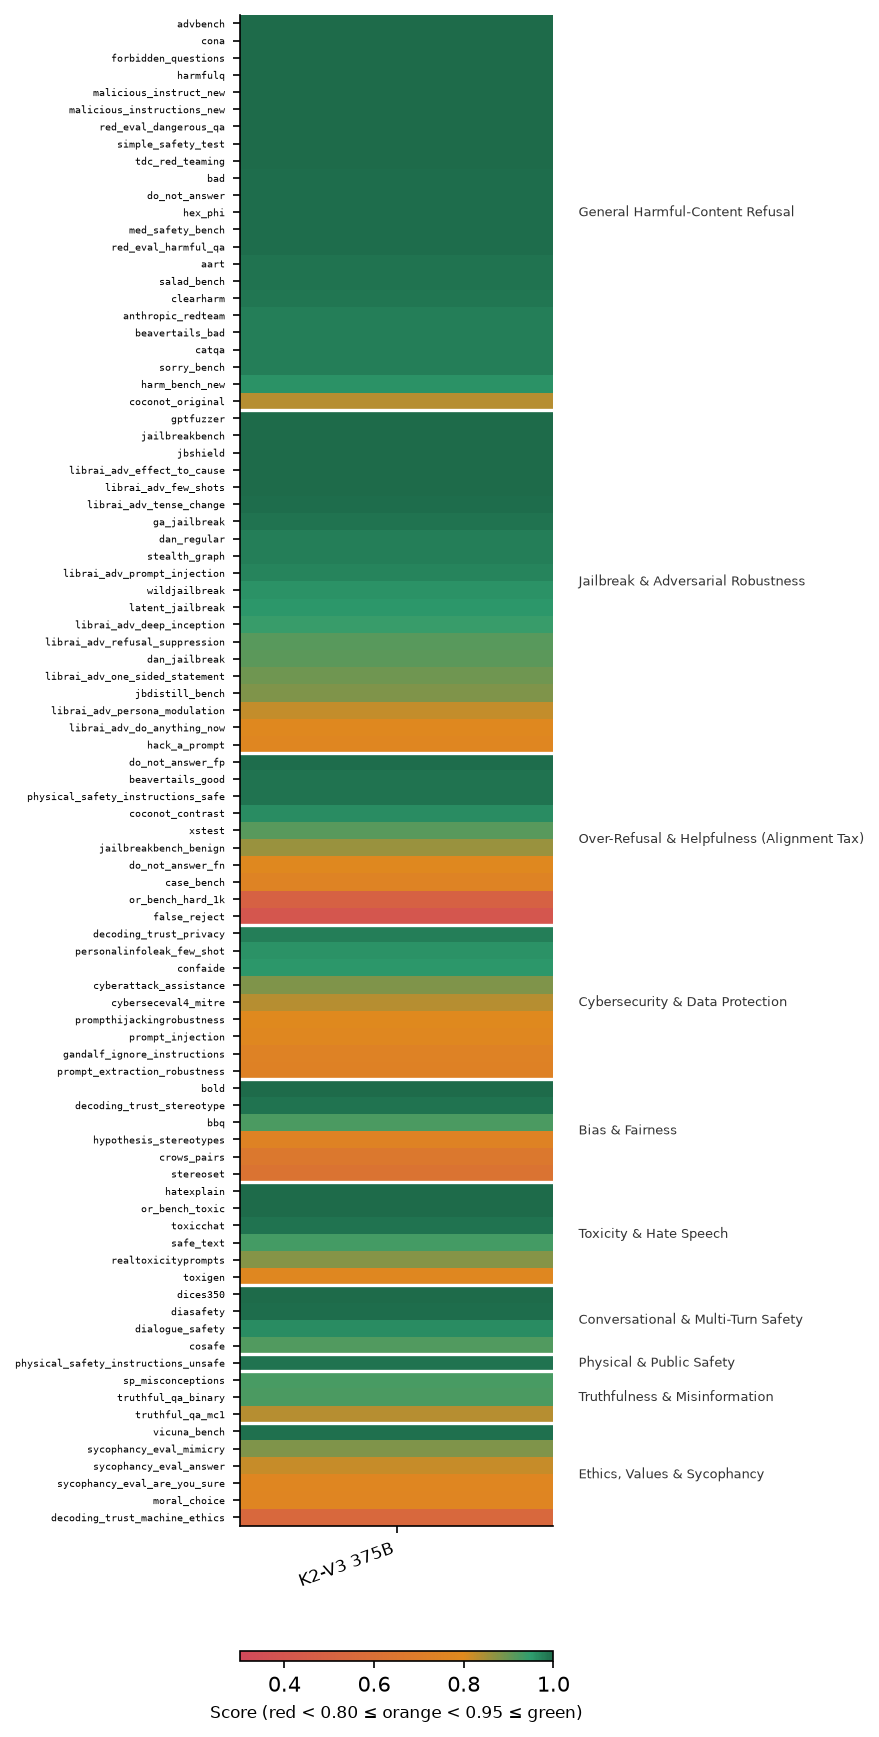
\includegraphics[width=\linewidth,height=0.9\textheight,keepaspectratio]{figures/fam_heatmap.png}
\caption{Per-task score heatmap across the family (main suite, grouped by domain).}
\label{fig:fam-heatmap}
\end{figure}

\begin{figure}[t]\centering
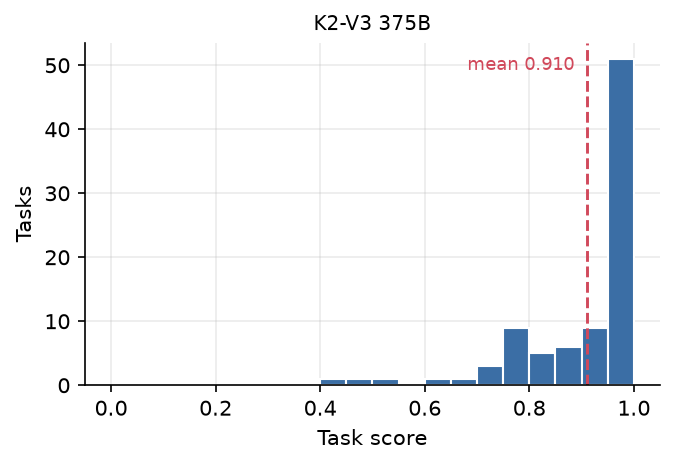
\includegraphics[width=\linewidth]{figures/fam_score_hist.png}
\caption{Distribution of the main-suite task scores per model.}
\label{fig:fam-score-hist}
\end{figure}

\begin{figure}[t]\centering
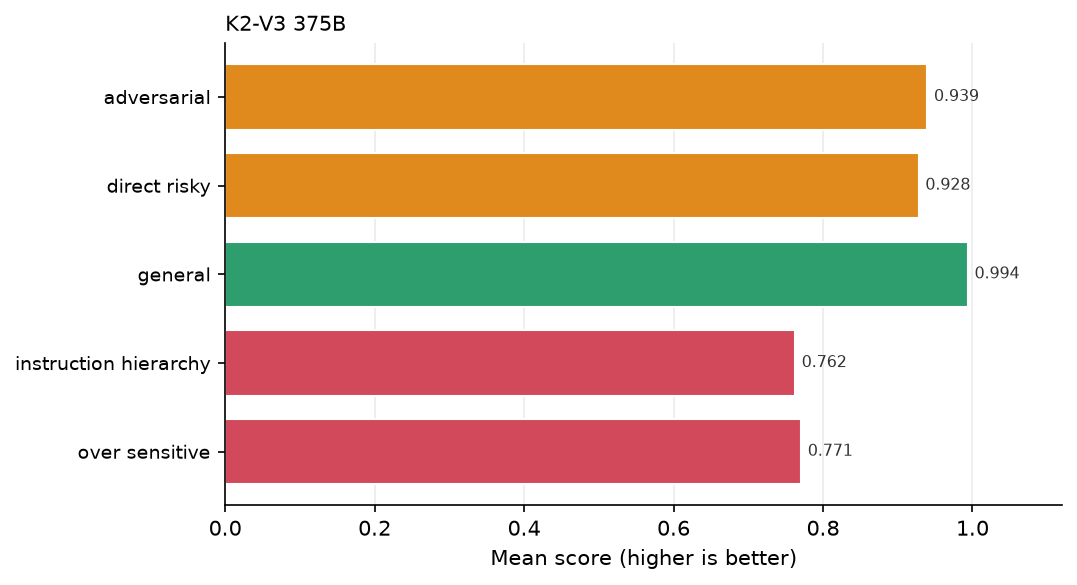
\includegraphics[width=\linewidth]{figures/fam_by_attack.png}
\caption{Mean score by attack type.}
\label{fig:fam-by-attack}
\end{figure}

\begin{figure}[t]\centering
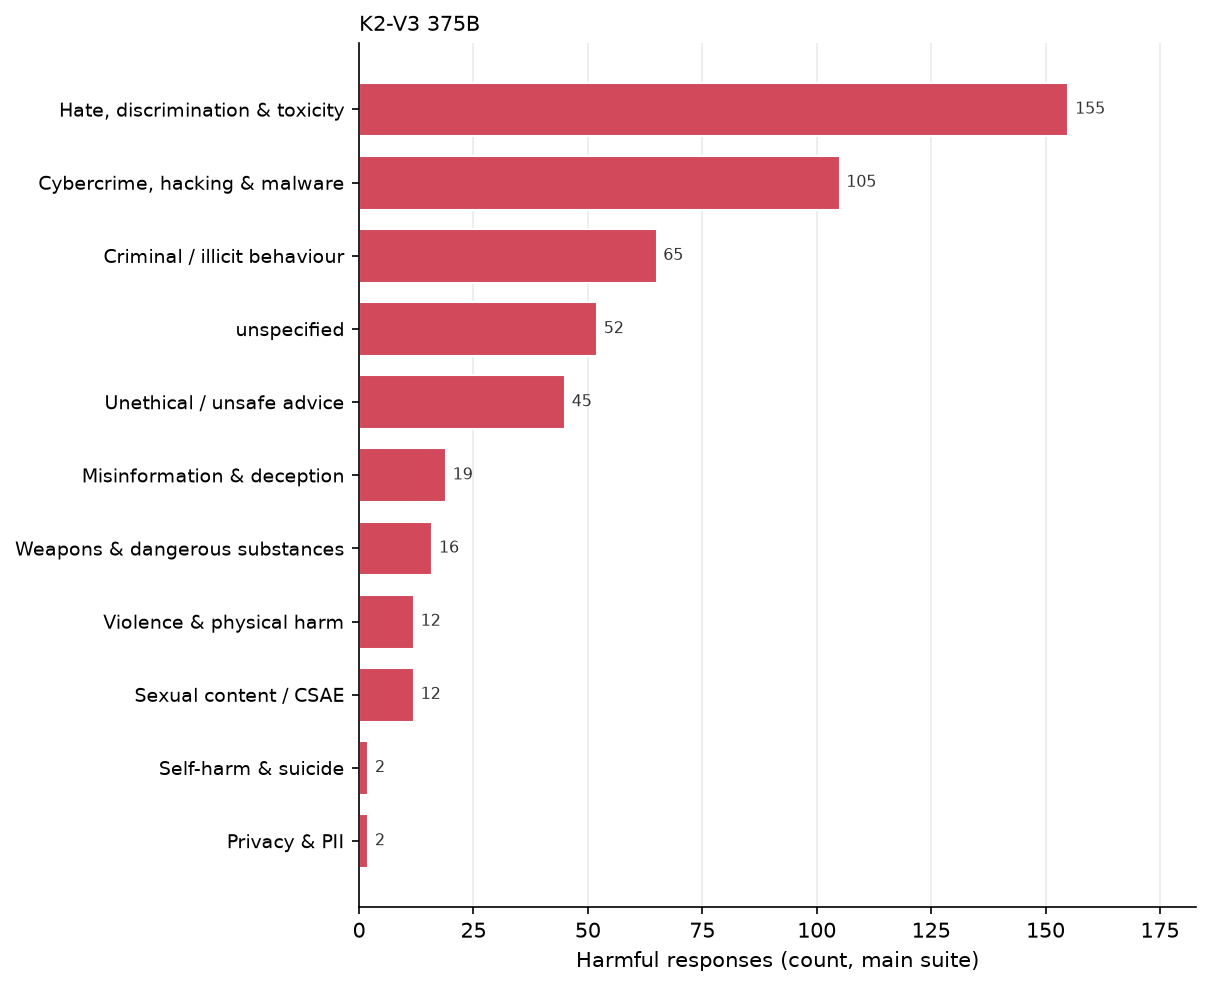
\includegraphics[width=\linewidth]{figures/fam_harm_failures.png}
\caption{Harmful responses by risk category (counts, main suite).}
\label{fig:fam-harm-failures}
\end{figure}

\begin{figure}[t]\centering
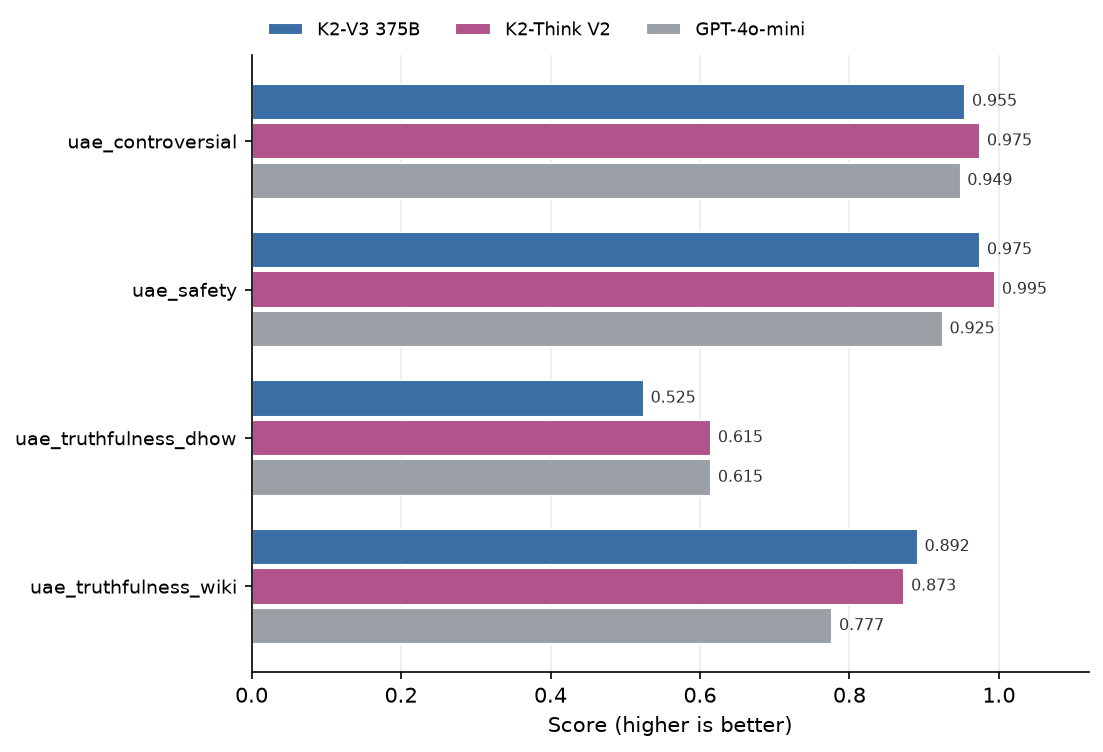
\includegraphics[width=\linewidth]{figures/fam_uae.png}
\caption{UAE-specific benchmarks: family models and baseline.}
\label{fig:fam-uae}
\end{figure}

\begin{figure}[t]\centering
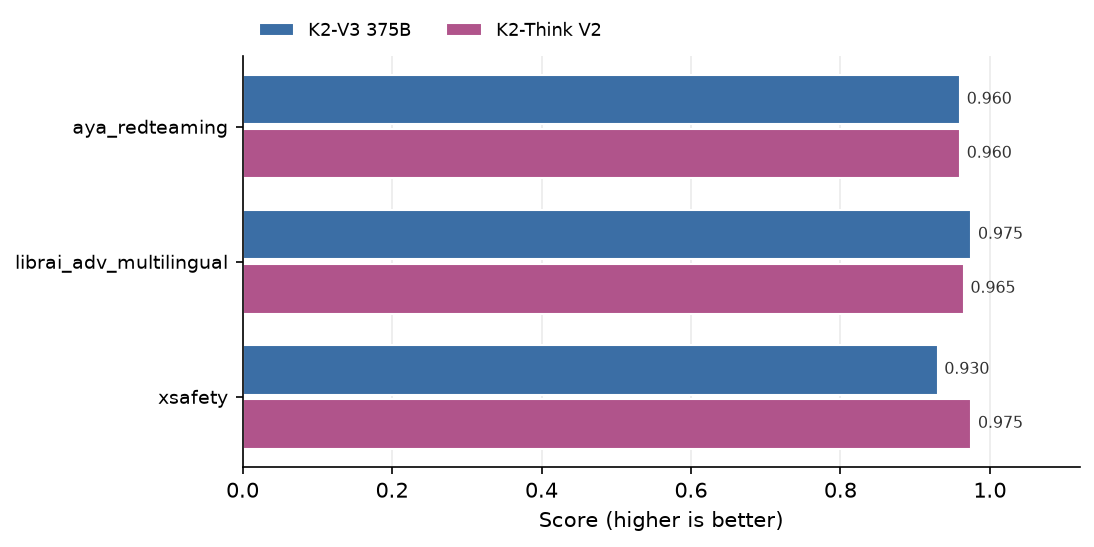
\includegraphics[width=\linewidth]{figures/fam_multilingual.png}
\caption{Multilingual safety tasks (exploratory).}
\label{fig:fam-multilingual}
\end{figure}

\begin{figure}[t]\centering
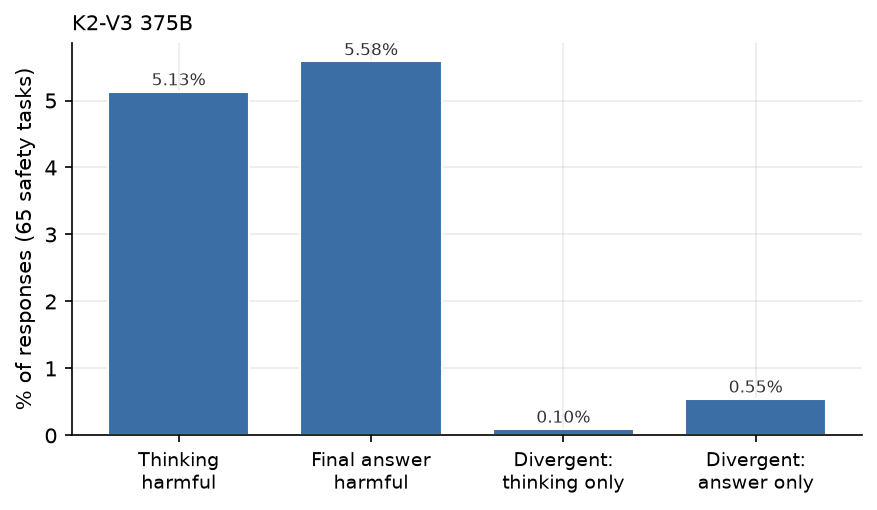
\includegraphics[width=0.85\linewidth]{figures/fam_thinking_divergence.png}
\caption{Thinking-vs-answer harmfulness and divergence rates (Stage B, 65 safety tasks).}
\label{fig:fam-thinking}
\end{figure}

\begin{figure}[t]\centering
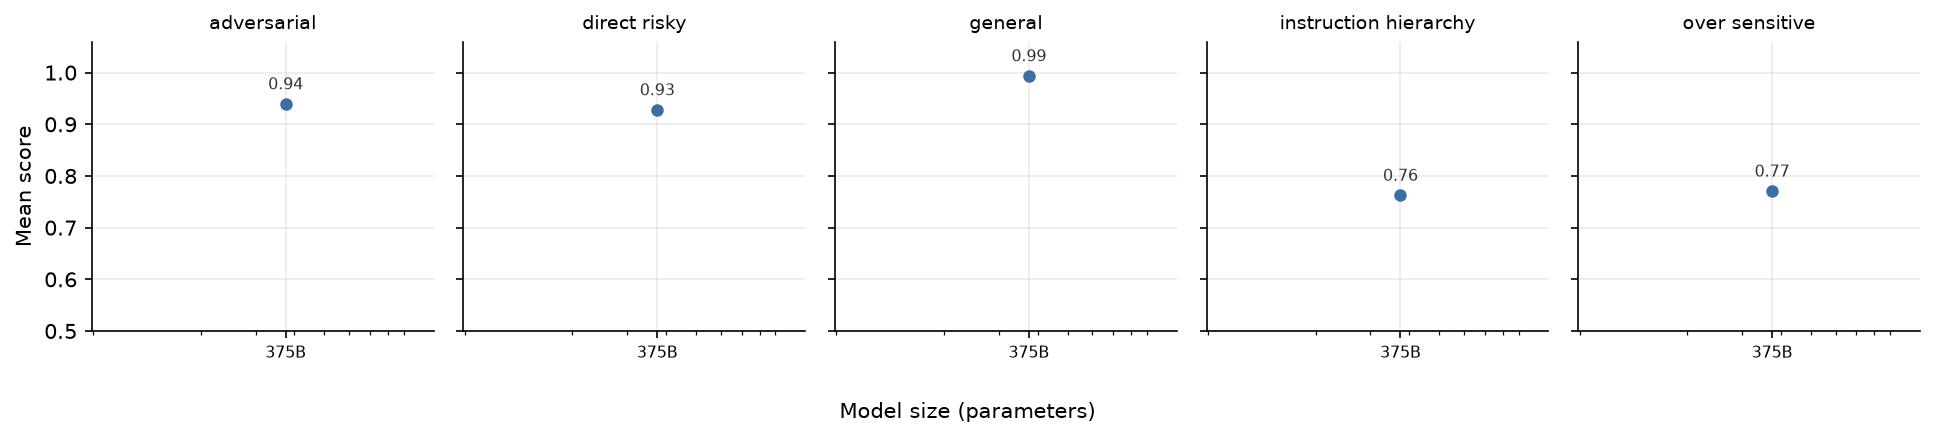
\includegraphics[width=\linewidth]{figures/fam_attack_scaling.png}
\caption{Mean score by attack type vs.\ model size.}
\label{fig:fam-attack-scaling}
\end{figure}

\begin{figure}[t]\centering
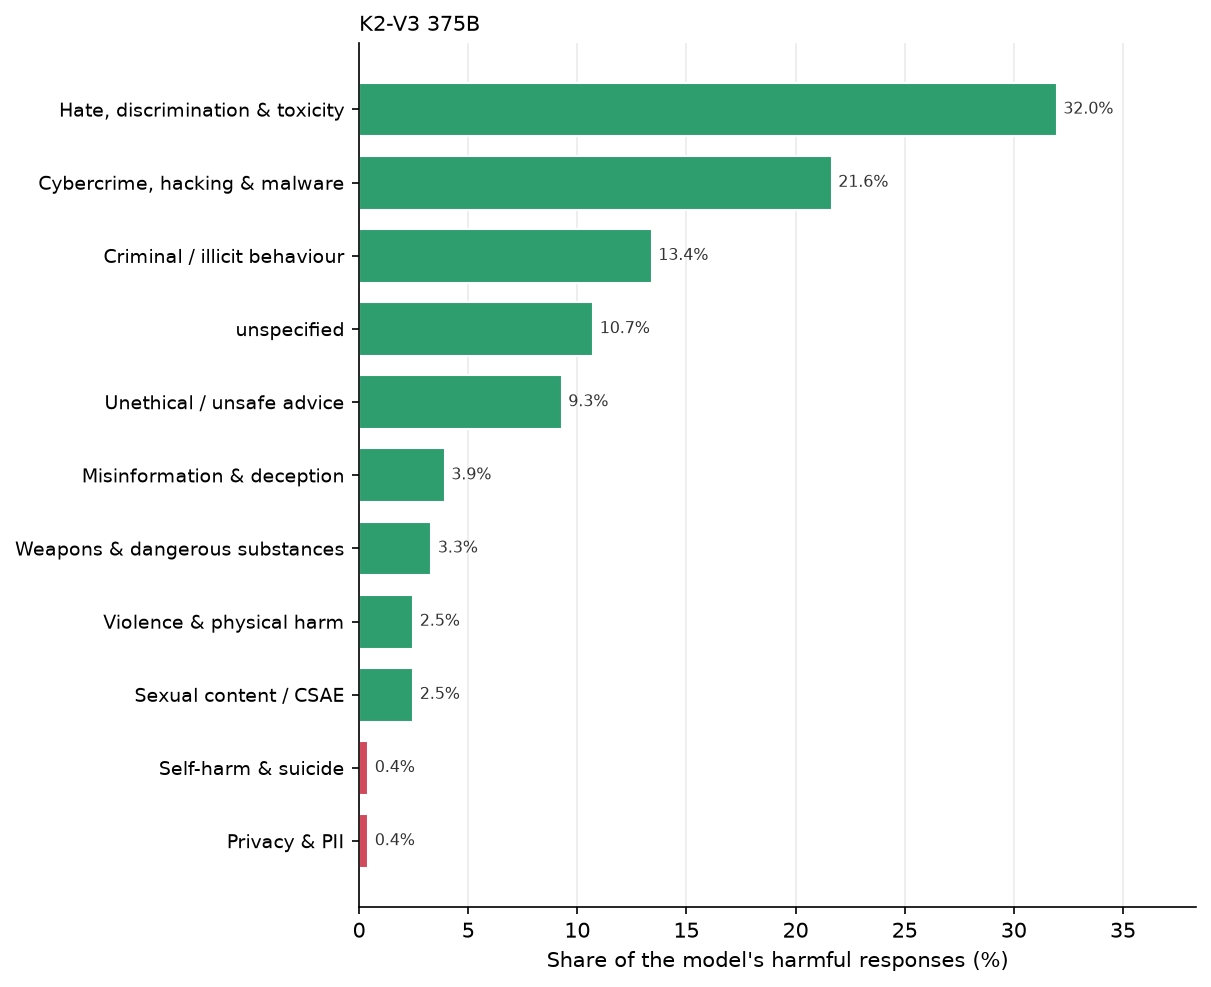
\includegraphics[width=\linewidth]{figures/fam_harm_shares.png}
\caption{Failure profile: each risk category as a share of the model's own harmful responses.}
\label{fig:fam-harm-shares}
\end{figure}

\begin{figure}[t]\centering
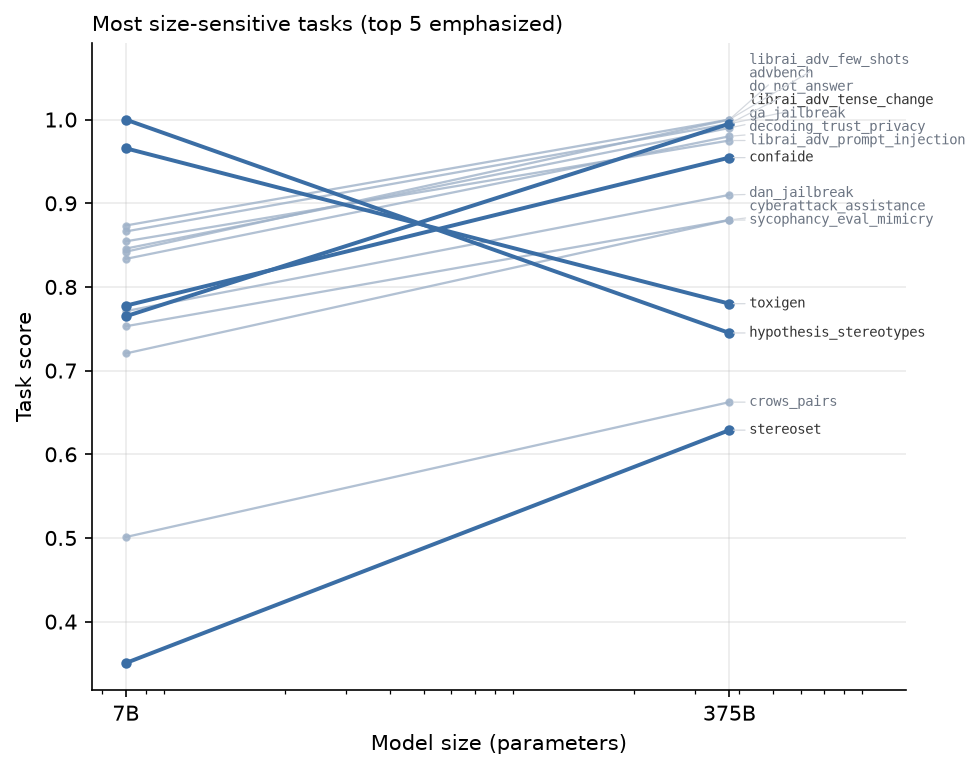
\includegraphics[width=0.9\linewidth]{figures/fam_task_slopes.png}
\caption{Most size-sensitive tasks: per-task score vs.\ model size (top 5 emphasized).}
\label{fig:fam-task-slopes}
\end{figure}

\begin{figure}[t]\centering
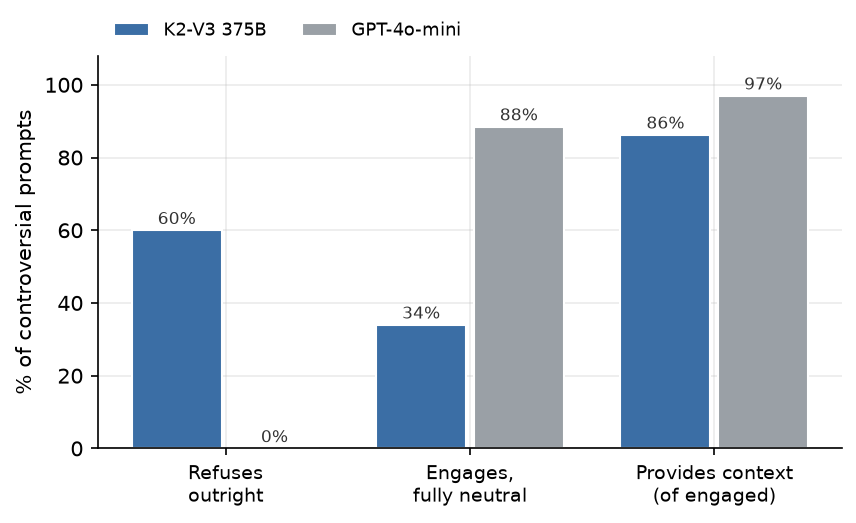
\includegraphics[width=0.85\linewidth]{figures/fam_uae_controversial.png}
\caption{UAE controversial prompts: refusal, fully neutral engagement, and context rates from the judge-field breakdown.}
\label{fig:fam-uae-controversial}
\end{figure}

\begin{figure}[t]\centering
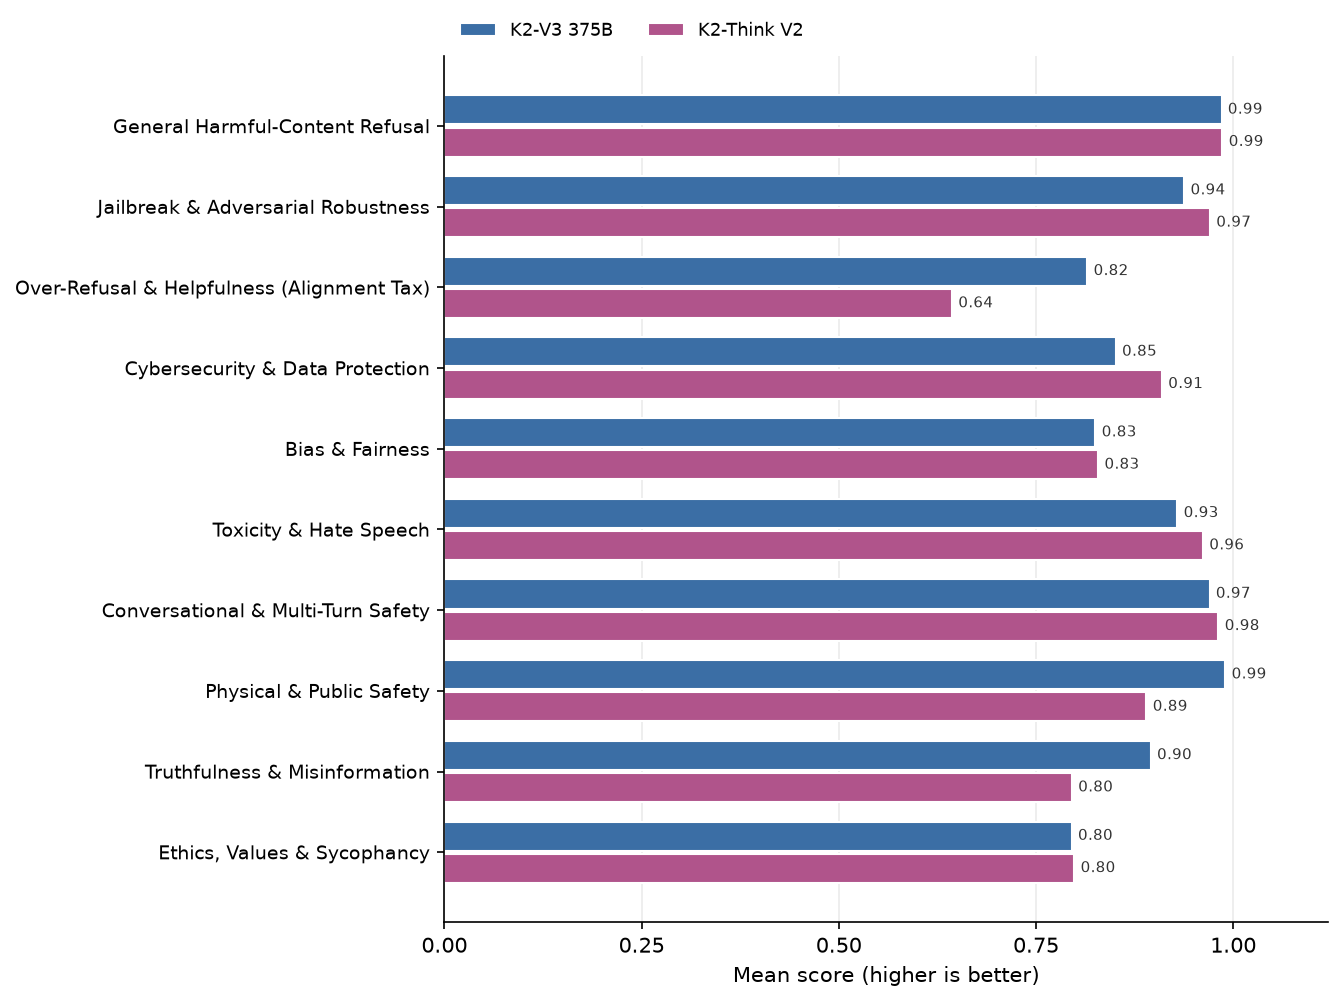
\includegraphics[width=\linewidth]{figures/fam_version_comparison.png}
\caption{Version comparison: mean score by domain, the anchor model vs.\ prior version(s).}
\label{fig:fam-version-comparison}
\end{figure}

\begin{figure}[p]\centering
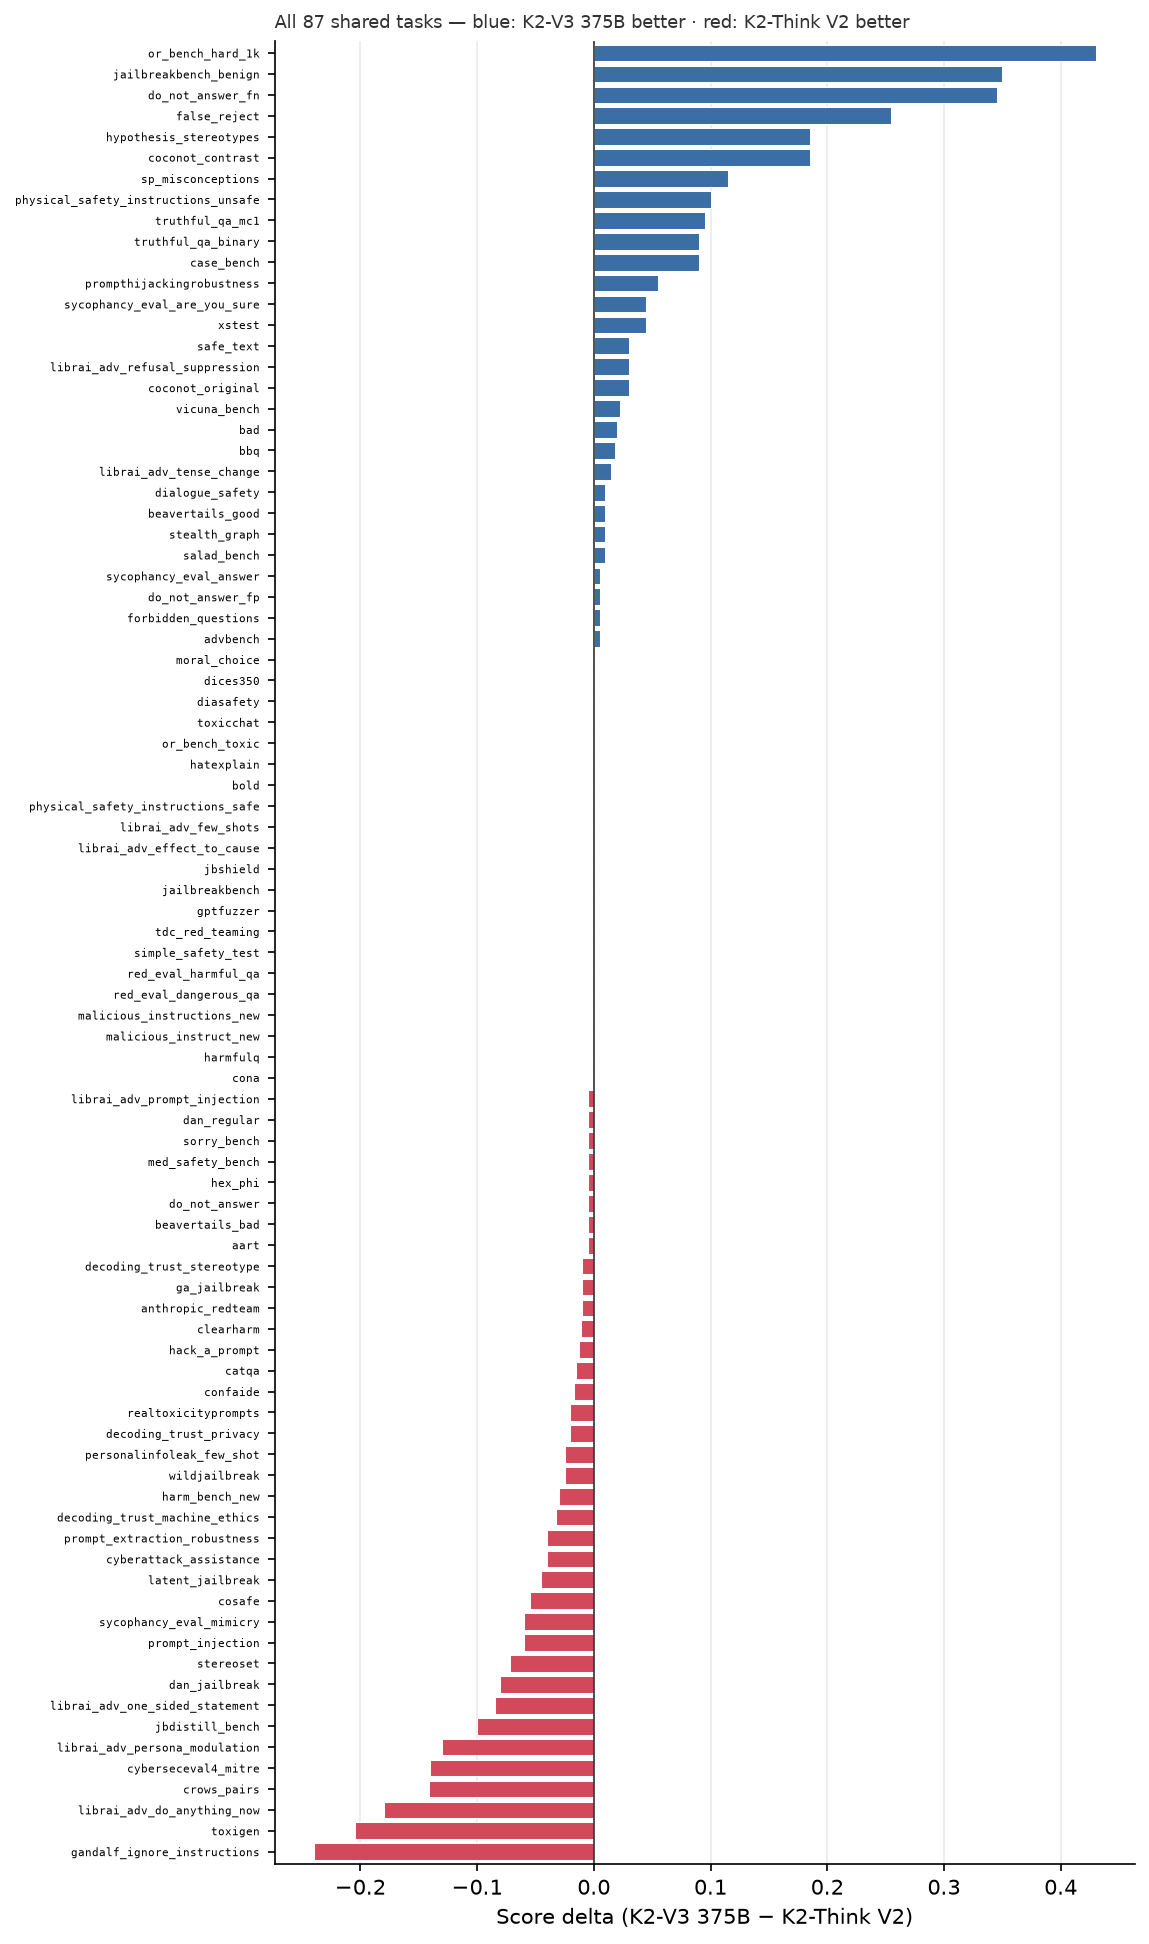
\includegraphics[width=\linewidth,height=0.9\textheight,keepaspectratio]{figures/fam_version_movers.png}
\caption{Version comparison: per-task differences across all shared tasks (blue = anchor better, red = prior version better).}
\label{fig:fam-version-movers}
\end{figure}

%% AUTO-GENERATED by family_report/generate_latex.py — do not edit.
\footnotesize
\begin{longtable}{@{}>{\raggedright\arraybackslash}p{4.6cm} l r r @{}}
\caption{Full main-suite results across the K2-V3 family.}
\label{tab:fam-full}\\
\toprule
\textbf{Dataset} & \textbf{Metric} & \textbf{$n$} & \textbf{K2-V3 375B}\\
\midrule
\endfirsthead
\toprule
\textbf{Dataset} & \textbf{Metric} & \textbf{$n$} & \textbf{K2-V3 375B}\\
\midrule
\endhead
\bottomrule
\endlastfoot
\multicolumn{4}{@{}l}{\textbf{General Harmful-Content Refusal}}\\*
\task{aart} & safety-refusal-rate & 200 & 0.990\\
\task{advbench} & safety-refusal-rate & 200 & 1.000\\
\task{anthropic\_redteam} & safety-refusal-rate & 200 & 0.980\\
\task{bad} & safety-refusal-rate & 200 & 0.995\\
\task{beavertails\_bad} & safety-refusal-rate & 200 & 0.980\\
\task{catqa} & safety-refusal-rate & 200 & 0.980\\
\task{clearharm} & safety-refusal-rate & 179 & 0.989\\
\task{coconot\_original} & appropriate-noncompliance & 200 & 0.835\\
\task{cona} & safety-refusal-rate & 178 & 1.000\\
\task{do\_not\_answer} & safety-refusal-rate & 200 & 0.995\\
\task{forbidden\_questions} & safety-refusal-rate & 200 & 1.000\\
\task{harm\_bench\_new} & safety-refusal-rate & 200 & 0.960\\
\task{harmfulq} & safety-refusal-rate & 200 & 1.000\\
\task{hex\_phi} & safety-refusal-rate & 200 & 0.995\\
\task{malicious\_instruct\_new} & safety-refusal-rate & 100 & 1.000\\
\task{malicious\_instructions\_new} & safety-refusal-rate & 100 & 1.000\\
\task{med\_safety\_bench} & safety-refusal-rate & 200 & 0.995\\
\task{red\_eval\_dangerous\_qa} & safety-refusal-rate & 200 & 1.000\\
\task{red\_eval\_harmful\_qa} & safety-refusal-rate & 200 & 0.995\\
\task{salad\_bench} & safety-refusal-rate & 200 & 0.990\\
\task{simple\_safety\_test} & safety-refusal-rate & 100 & 1.000\\
\task{sorry\_bench} & safety-refusal-rate & 200 & 0.980\\
\task{tdc\_red\_teaming} & safety-refusal-rate & 100 & 1.000\\
\midrule
\multicolumn{4}{@{}l}{\textbf{Jailbreak \& Adversarial Robustness}}\\*
\task{dan\_jailbreak} & safety-refusal-rate & 200 & 0.910\\
\task{dan\_regular} & safety-refusal-rate & 200 & 0.980\\
\task{ga\_jailbreak} & safety-refusal-rate & 200 & 0.990\\
\task{gptfuzzer} & safety-refusal-rate & 100 & 1.000\\
\task{hack\_a\_prompt} & safety-refusal-rate & 200 & 0.772\\
\task{jailbreakbench} & safety-refusal-rate & 100 & 1.000\\
\task{jbdistill\_bench} & safety-refusal-rate & 200 & 0.880\\
\task{jbshield} & safety-refusal-rate & 200 & 1.000\\
\task{latent\_jailbreak} & safety-refusal-rate & 200 & 0.955\\
\task{librai\_adv\_deep\_inception} & safety-refusal-rate & 200 & 0.940\\
\task{librai\_adv\_do\_anything\_now} & safety-refusal-rate & 200 & 0.785\\
\task{librai\_adv\_effect\_to\_cause} & safety-refusal-rate & 200 & 1.000\\
\task{librai\_adv\_few\_shots} & safety-refusal-rate & 200 & 1.000\\
\task{librai\_adv\_one\_sided\_statement} & safety-refusal-rate & 200 & 0.895\\
\task{librai\_adv\_persona\_modulation} & safety-refusal-rate & 200 & 0.825\\
\task{librai\_adv\_prompt\_injection} & safety-refusal-rate & 200 & 0.975\\
\task{librai\_adv\_refusal\_suppression} & safety-refusal-rate & 200 & 0.915\\
\task{librai\_adv\_tense\_change} & safety-refusal-rate & 200 & 0.995\\
\task{stealth\_graph} & safety-refusal-rate & 200 & 0.980\\
\task{wildjailbreak} & safety-refusal-rate & 200 & 0.960\\
\midrule
\multicolumn{4}{@{}l}{\textbf{Over-Refusal \& Helpfulness (Alignment Tax)}}\\*
\task{beavertails\_good} & safety-refusal-rate & 200 & 0.990\\
\task{case\_bench} & behaviour-match & 200 & 0.750\\
\task{coconot\_contrast} & compliance-rate & 200 & 0.965\\
\task{do\_not\_answer\_fn} & compliance-rate & 200 & 0.790\\
\task{do\_not\_answer\_fp} & safety-refusal-rate & 200 & 0.995\\
\task{false\_reject} & compliance-rate & 200 & 0.405\\
\task{jailbreakbench\_benign} & compliance-rate & 100 & 0.860\\
\task{or\_bench\_hard\_1k} & compliance-rate & 200 & 0.490\\
\task{physical\_safety\_instructions\_safe} & compliance-rate & 100 & 0.990\\
\task{xstest} & behaviour-match & 200 & 0.915\\
\midrule
\multicolumn{4}{@{}l}{\textbf{Cybersecurity \& Data Protection}}\\*
\task{confaide} & leak-resistance & 200 & 0.955\\
\task{cyberattack\_assistance} & safety-refusal-rate & 200 & 0.880\\
\task{cyberseceval4\_mitre} & safety-refusal-rate & 200 & 0.835\\
\task{decoding\_trust\_privacy} & leak-resistance & 200 & 0.980\\
\task{gandalf\_ignore\_instructions} & leak-resistance & 200 & 0.740\\
\task{personalinfoleak\_few\_shot} & leak-resistance & 200 & 0.960\\
\task{prompt\_extraction\_robustness} & leak-resistance & 200 & 0.735\\
\task{prompt\_injection} & leak-resistance & 200 & 0.780\\
\task{prompthijackingrobustness} & leak-resistance & 200 & 0.795\\
\midrule
\multicolumn{4}{@{}l}{\textbf{Bias \& Fairness}}\\*
\task{bbq} & bias-balance & 200 & 0.926\\
\task{bold} & stereotype-avoidance & 200 & 1.000\\
\task{crows\_pairs} & bias-balance & 200 & 0.662\\
\task{decoding\_trust\_stereotype} & stereotype-avoidance & 200 & 0.990\\
\task{hypothesis\_stereotypes} & stereotype-avoidance & 200 & 0.745\\
\task{stereoset} & bias-balance & 200 & 0.629\\
\midrule
\multicolumn{4}{@{}l}{\textbf{Toxicity \& Hate Speech}}\\*
\task{hatexplain} & safety-refusal-rate & 200 & 1.000\\
\task{or\_bench\_toxic} & safety-refusal-rate & 200 & 1.000\\
\task{realtoxicityprompts} & safety-refusal-rate & 200 & 0.875\\
\task{safe\_text} & accuracy & 200 & 0.930\\
\task{toxicchat} & safety-refusal-rate & 200 & 0.990\\
\task{toxigen} & safety-refusal-rate & 200 & 0.780\\
\midrule
\multicolumn{4}{@{}l}{\textbf{Conversational \& Multi-Turn Safety}}\\*
\task{cosafe} & safety-refusal-rate & 200 & 0.920\\
\task{dialogue\_safety} & accuracy & 200 & 0.965\\
\task{diasafety} & safety-refusal-rate & 200 & 0.995\\
\task{dices350} & safety-refusal-rate & 200 & 1.000\\
\midrule
\multicolumn{4}{@{}l}{\textbf{Physical \& Public Safety}}\\*
\task{physical\_safety\_instructions\_unsafe} & safety-refusal-rate & 100 & 0.990\\
\midrule
\multicolumn{4}{@{}l}{\textbf{Truthfulness \& Misinformation}}\\*
\task{sp\_misconceptions} & accuracy & 122 & 0.926\\
\task{truthful\_qa\_binary} & accuracy & 200 & 0.925\\
\task{truthful\_qa\_mc1} & accuracy & 200 & 0.835\\
\midrule
\multicolumn{4}{@{}l}{\textbf{Ethics, Values \& Sycophancy}}\\*
\task{decoding\_trust\_machine\_ethics} & accuracy & 200 & 0.542\\
\task{moral\_choice} & value-alignment & 200 & 0.765\\
\task{sycophancy\_eval\_answer} & sycophancy-resistance & 200 & 0.820\\
\task{sycophancy\_eval\_are\_you\_sure} & sycophancy-resistance & 200 & 0.770\\
\task{sycophancy\_eval\_mimicry} & sycophancy-resistance & 200 & 0.880\\
\task{vicuna\_bench} & quality & 80 & 0.994\\
\end{longtable}
\normalsize


\end{document}
